\chapter{The Kakeya Problem in Finite Fields \label{chap:kakeya}}
Before we can discuss the Kakeya problem in finite fields, and its rather surprising resolution, we ought to first discuss the origin and history of the problem. 
Work on the Kakeya problem can be traced back to the Russian mathematician Abram Besicovitch in 1917. While working on a problem in Riemann integration, Besicovitch reduced it to the question
of the existence of planar sets of measure zero which contain a line segment in every direction. In 1920, Besicovitch constructed such a set and published in a Russian Journal.

However, 1917 was a turbulent year as it marked the end of
the Russian Empire and the start of the Russian civil war. Due to this and the ensuing blockade of Russian ports there was scarce communication with the outside world.
Thus Besicovitch could not have known of a Japanese mathematician Kakeya who asked also in 1917 a related question: What is the smallest area of a convex set within which
one can rotate a needle by 180 degrees in the plane? Julius Pal answered this question in 1921 with the equilateral triangle. The 
more interesting problem without the convexity condition remained open. In 1924, after leaving the newly formed Soviet Union for Copenhagen, Besicovitch discovered this
problem and by modifying his previous construction produced a solution in 1925. This lead to the more general questions being asked about Kakeya sets in higher dimensions.
\begin{definition}[Kakeya Set in $\RR^n$]
    A Kakeya set is a set $A \subset \RR^n$ that contains a unit segment in every direction.
\end{definition}
Besicovitch's construction showed that these sets can have arbitrarily small measures, even attaining zero, in $\RR^2$. Further, a straightforward construction produces these measure zero sets in dimensions $> 2$.

The natural question then arises, what is the dimension of such sets? There are many notions of dimensions that can be investigated, but we restrict ourselves to the Minkowski and Hausdorff dimensions.

\begin{definition}[Minkowski Dimension]
Given a set $S \subset \RR^n$, define $N(\varepsilon)$ to be the number of boxes of side length $\varepsilon$ required to cover the set.
The Minkowski Dimension of the set $S$ is then defined as:
$$\dim_M (S) = \lim_{\varepsilon \to 0} \frac{\log( N(\varepsilon))}{\log (1/\varepsilon)}.$$
If this limit does not exist, one can still define the upper and lower Minkowski dimensions, 
$\dim_{M_{\text{upper}}}$ and $\dim_{M_{\text{lower}}}$, by taking the limit superior and limit inferior respectively.
\end{definition}
\begin{definition}[Hausdorff Dimension]
    We define the $d$-dimensional Hausdorff measure of a set $S \subset \RR^n$ as: 
    $$\mathcal{H}^d(S)=\lim_{r \to 0} \inf \left\{\sum_i r_i^d:\text{ there is a countable cover of } S\text{ by balls with radii } 0 < r_i < r\right\}$$
    Then we can define the Hausdorff dimension of the set $S$ to be:
    $$\dim_H (S) = \inf \{ d \geq 0 : \mathcal{H}^d(S) = 0 \}.   $$
\end{definition}
These dimensions are related by the following inequality when they are all defined:
$$\dim_H \leq \dim_{M_{\text{lower}}} \leq \dim_{M_{\text{upper}}}.$$
In 1971, Davies produced a solution for the 2 dimensional case, proving that
although the measure of a Kakeya set can be arbitrarily small, it must have Hausdorff and Minkowski dimension of 2.\cite{davies1971some}
This resulted in the following conjectures:
\begin{conjecture}[Kakeya Conjecture for the Minkowski Dimension]
    Let $A$ be a Kakeya set in $\RR^n$. Then $\dim_M (A) = n$. \label{conj:mink-kakeya}
\end{conjecture}
\begin{conjecture}[Kakeya Conjecture for the Hausdorff Dimension]
    Let $A$ be a Kakeya set in $\RR^n$. Then $\dim_H (A) = n$. \label{conj:haus-kakeya}
\end{conjecture}
In a survey on the problem, Wolff proposed a finite analogue to the Kakeya Conjecture.\cite{wolff1999recent} 

A Kakeya set in $\FP^n$ is a set that contains a line in every direction. Analogous to the Euclidean case, we formally define lines in $\FP^n$  as the set:
$$\mathcal{L} = \{x+ty : x,y \in \FP^n,  t \in \FP \}.$$
It should be noted that a line in a finite field $\FP^n$ contains exactly $|\FP|$ points.
Formally, directions in $\FP^n$ can be identified using the projective space $\mathbb{P}\FP^n  = \frac{\FP^n}{\FP^x}$.
The finite analogue to Conjectures \ref{conj:mink-kakeya} and \ref{conj:haus-kakeya} is:
\begin{theorem}[Kakeya Conjecture in Finite Fields]
    If $A\subset \FP^n$ contains a translate of every line, then $|A| \geq \frac{1}{n!} |\FP|^n $. \label{KakeyaConjecture}
\end{theorem}
This conjecture had a significant influence on the subject, inspiring work on the sum-product phenomenon in finite fields. From its postulation in 1999,
little progress was made in the following years and it was assumed that the problem was roughly as difficult as the Euclidean case. 

In 2008, Dvir published a remarkably simple proof of Theorem \ref{KakeyaConjecture} using basic facts about polynomials. 
This proof revitalised interest in the polynomial method, and we shall explore its details later in this chapter. 

\begin{figure}[h]
\centering 
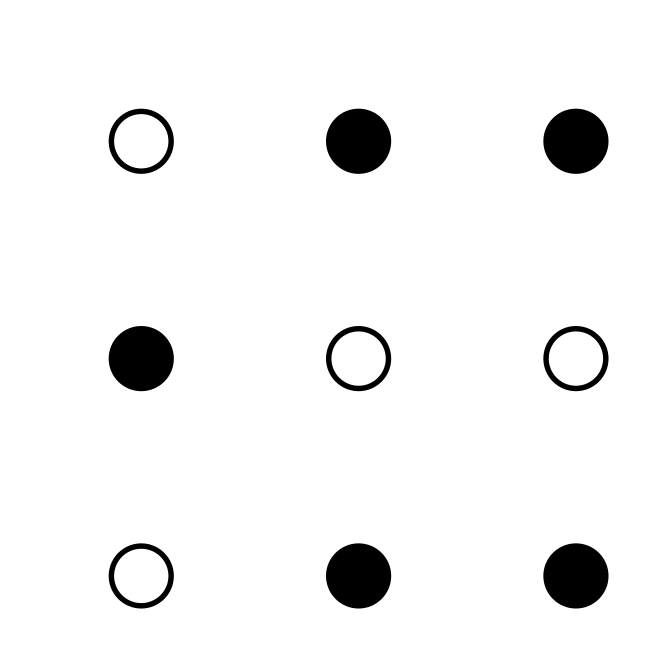
\includegraphics[width=0.3\textwidth]{images/kakeya_ex_f32.png}}
\caption{An example of a Kakeya set (shaded) in $\FF_3^2$.}
{\label{kak_ex_f32}
\end{figure}
\todo{big example}


\section{Introduction to Finite Fields}
\begin{definition}[Finite Field]
    A finite field, $\FF$, is a finite set that forms a field. That is, it is closed under addition, subtraction, multiplication, and non-zero division. 
    The number of elements of a finite field, $|\FF|$, is called the order of the finite field.
\end{definition}
A finite field of order $q$ exists if and only if $q = p^k$ for some prime $p$ and integer $k$. 

\begin{lemma}
    Each element $X$ in a finite field $\FF$ satisfies the identity:
    $$X^{|\FF|} - X =0$$
    identically in $\FF$. \label{lem:finite-fields-poly-identity}
\end{lemma}
This lemma follows immediately from Fermat's Little Theorem.




\section{Combinatorial Attempts }
To truly show the power of the polynomial method, we shall first explore purely combinational attempts 
at estimating the sizes of Kakeya sets. All of the following estimates are much weaker than the bound in Theorem \ref{KakeyaConjecture}.
We fix a finite field $\FF = \FF_{p^k}$ where $p$ is a prime. 

Our first estimate gives a good bound for the $n$ = 2 case for the finite field Kakeya problem.

\begin{lemma}
    Suppose $s<|\FF|$. If $l_1, \dots, l_s$ are distinct lines in $\FF^n$, then their union has cardinality at least $(1/2)|\FF|s$. 

    In particular, if $A \subset \FF^n$ is a Kakeya set, then we have:
    \[
      |A| \gtrsim |\FF|^2  
    \] \label{lem:kak-first-estimate}
\end{lemma} 
\begin{proof}
    We add the lines one at a time and track the cardinality of their union. The first line contains $|\FF|$ points. The second line must contain at least $|\FF| -1$ points not in the first line. Similarly the third line must contain at least $|\FF| -2$ points not in the first two lines, and so on. Thus the number of distinct points in the union of all $s$ lines is given by:
    \[
      \sum_{i=1}^{s} |\FF| - i + 1  > (1/2) |\FF| s.
    \]

    A Kakeya set always contains at least $|\FF|$ lines, so setting $s=|\FF|$ above yields:
    \[
        |A| > (1/2) |\FF|^2 
    \]

\end{proof}

\subsection{Bush Argument} 
Bourgain produced one of the first non-trivial estimates of the dimension in 1991.\cite{BUSH1991} We present the finite field analogue of his argument here.\cite{GUTH2016}
\begin{theorem}[Bush Argument]

If $A$ is a Kakeya set, then we have:
$$|A| \gtrsim |\FF|^{\frac{n+1}{2}}$$
\end{theorem}

\begin{proof}
    Let $\mu$ be a fixed multiplicity parameter to be chosen later. Then either there exists a point $p\in A$ such that there are $\mu$ lines passing through $p$,
    or else every point in $A$ has less than $\mu$ lines passing through it.

    In the first case, since the lines have distinct directions they must become disjoint when $p$ is removed. Hence,
    \[
      |A| \gtrsim \mu |\FF| .
    \]

    In the latter case, by considering the double sum and double counting:
    \begin{align*}
         \sum_{\ell \in K} \sum_{p \in A} \OO[p \in \ell] &= \sum_{\ell \in K} |\FF| = |\FF|^{n-1} |\FF| \\
        \sum_{p \in A} \sum_{\ell \in K} \OO[p \in \ell] &\leq \sum_{p \in A} \mu = |A|\mu \\
        \implies \frac{|\FF|^{n}}{\mu} \leq |A|.
    \end{align*}
    Now optimising $\mu$:
    \begin{align*}
        \frac{|\FF|^{n}}{\mu} &\sim \mu |\FF| \\
        \mu &\sim |\FF|^{\frac{n-1}{2}}.
    \end{align*}
    This yields the bound:
    \[
        |A| \gtrsim |\FF||\FF|^{\frac{n-1}{2}} \sim |\FF|^{\frac{n+1}{2}}.
    \]

\end{proof}

\subsection{Hairbrush Argument}
Due to Wolff. \cite{WOLFF1995}

\begin{theorem}[Hair Brush Argument]
    If $A$ is a Kakeya set, then we have:
    \[
        |A| \gtrsim |\FF|^{\frac{n+2}{2}}    
    \]
\end{theorem}
\begin{proof}
By Lemma \ref{lem:kak-first-estimate}, if $A_m \subset \FF^2$ is a set containing a line in $m$ different directions then $|A_m| \gtrsim m|\FF|$.

Let $\mu$ be a fixed multiplicity parameter to be chosen later. We say a line $\ell$ is $\mu$-rich if for at least $|\FF|/2$ points $p\in \ell$ there are $\mu$ lines distinct from $p$
in $A$ passing through $p$. Then either there exists a $\mu$-rich line or there does not. 

Suppose a $\mu$-rich line exists, and denote this line by $\ell_\mu$. Consider the family of 2-dimensional planes $\Pi$ passing through $\ell_\mu$. 
If a line $\ell$ intersects $\ell_\mu$ then there exists a unique plane $\pi \in \Pi$ such that $\ell, \ell_\mu \in \pi$. 
Let $\LL_\pi := \{\ell \subset \pi \ | \ \ell \cap \ell_\mu \neq \emptyset \}$. The set $A \cap \pi$ is a set in $\FF^2$ that contains at least $|\LL_\pi|$
lines, and hence by Lemma \ref{lem:kak-first-estimate} we have:
\[
|A \cap \pi| \gtrsim |\LL_\pi| |\FF|.
\]
Thus,
\[
    |A| \geq \sum_{\pi \in \Pi} |(A \cap \pi) \backslash \ell_\mu| \gtrsim |\FF| \sum_{\pi \in \Pi} |\LL_\pi| \gtrsim \mu |\FF|^2,
\]
where the last inequality comes from the fact $\ell_\mu$ intersects at least $\mu |\FF|/2$ lines, which produces $\mu |\FF|/2$ planes as all these lines are distinct.

Suppose there does not exist a $\mu$-rich line. Let 
\[
    A' = \{p \in A \ | \ p \text{ belongs to at most } \mu \text{ lines in }A \}.
\]
Since we assume there does not exist a $\mu$-rich line in $A$, for any line $\ell \subset A$ we have $|A' \cap \ell| > |F|/2$. 
Proceeding by double counting, \todo{split this into two steps}
\begin{align*}
    |A| &\geq |A'|\geq \frac{1}{\mu} \sum_{p \in A'} \sum_{\ell \in A} \OO[p \in \ell] \\
    &= \frac{1}{\mu} \sum_{\ell \in A} |A' \cap \ell| \gtrsim \frac{1}{\mu} |\FF|^{n-1}|\FF|\\
    \implies |A| &\gtrsim \frac{|\FF|^n}{\mu}.
\end{align*}
We now optimise $\mu$:
\begin{align*}
    \frac{|\FF|^n}{\mu} &\sim \mu |\FF|^2 \\
    \mu &\sim |\FF|^{\frac{n-2}{2}}
\end{align*}
Thus we achieve the bound:
\[
    |A| \gtrsim |\FF|^2|\FF|^{\frac{n-2}{2}} \sim |\FF|^{\frac{n+2}{2}}.
\]
\end{proof}

\section{Dvir's Proof \label{sect:Dvirs-proof}}
We shall prove this theorem via 3 surprisingly simple lemmas. The general strategy of the proof is to assume a Kakeya set $A$ is of a limited size and find a low-degree non-zero polynomial that interpolates (contains in its zero set) the points in $A$. We then show that due to the structure of the Kakeya set the polynomial's zero set must contain many more points. This contradicts the fact our polynomial is non-zero and establishes the Kakeya Conjecture over finite fields.

\begin{lemma}[Parameter Counting] 
Let $\KK$ be a (not necessarily finite) field. If $A \subset \KK^n$ and $|A| < {{n+D} \choose {n}}$, there exists a non-zero polynomial $P(x_1,\dots, x_n)$ of degree $D$ that vanishes on $A$. \label{lem:paramcounting}
\end{lemma}

\prf{ We first show the dimension of $\text{Poly}_D (\KK^n)$ is ${D+n} \choose{n}$. A basis for $\text{Poly}_D (\KK^n)$ is given by monomials of the form $x_1^{D_1}\dots x_n^{D_n}$, where $\sum_i D_i \leq D$, hence we just need to count the number of monomials.

We can map a monomial $x_1^{D_1}\dots x_n^{D_n}$ to a string of $D$ $\star$'s and $n$ $|$'s as follows. 
Begin with $D_1$ $\star$'s, then place one $|$. We put now $D_2$ $\star$'s, and place a second $|$. 
We continue until we have placed $D_n$ $\star$'s followed by an $n^{\text{th}}$ $|$. 
Finally we place $D - \sum_i D_i \star$'s.
 This is a bijective map between the monomials in $\text{Poly}_D (\KK^n)$ and all the strings of $D$ $\star$'s and $n$ $|$'s. 
 To assemble such a string we distribute the $n$ $|$'s over $n+D$ spaces, and then fill the remainder with $\star$'s. Hence we get the binomial coefficient:
$$\text{Poly}_D (\KK^n) = {{n+D} \choose{n}}.$$

Now let $p_1, \dots, p_{|A|}$ be the points of $A$. We consider the evaluation map $E: \text{Poly}_D (\KK^n) \to \KK^{|A|}$ defined by:
$$E(Q) = \left(Q(p_1), \dots, Q(p_{|A|})\right).$$

This map is clearly linear. 
Its kernel $\ker E$ is exactly the set of polynomials in $\text{Poly}_D (\KK^n)$ that vanish on $A$. 
By assumption, the dimension of $\text{Poly}_D (\KK^n)$ is greater than $A$, so the dimension of the domain of $E$ is greater than the codomain of $E$. By the rank-nullity theorem, we conclude $E$ must have a non-trivial kernel. 
Thus there exists a non-zero polynomial $P \in \text{Poly}_D (\KK^n)$ that vanishes on $A$.} 


Note that if $D=|\FF|-1$, and $|A| \leq {{|\FF|+n-1} \choose{|\FF|-1}} = { {|\FF|+n-1} \choose{n}}$ we have a polynomial of degree $|\FF|-1$ that vanishes on $A$. Since $\frac{|\FF|^n}{n!} < {{|\FF|+n-1} \choose{n}}$,we can definitely find such a polynomial when $|A| \leq \frac{|\FF|^n}{n!}$.


\begin{lemma}Suppose $A \subset \FF^n$ contains a line in every direction, and suppose that there exists a non-zero polynomial $P$ with degree $D<|\FF|$ that vanishes on $A$. Then there exists a non-zero degree $D$ polynomial $\bar{P}$ that vanishes everywhere on $\FF^n$. \label{lem:kaklem2} \end{lemma}

\prf{ Choose a line in $A$, say $\ell = \{x+tz : t\in \FF \}$ with $x\in \FF^n$ and $z \in \FF^n / \FF^{\times}$. Now we consider the restriction of our polynomial $P$ to the line $\ell$, $P_{|\ell}$ .
Recall $P$ is a sum of monomials, and we use multi-index notation here with $\alpha = (\alpha_1, \alpha_2, \dots, \alpha_n), \ \alpha_i \in \NN \cup \{0\}$ and $|\alpha| =  \sum \alpha_i$. $P$ can be written as:
$$P(x_1,x_2, \dots, x_n) = \sum_{|\alpha| \leq D} c_{\alpha} x_1^{\alpha_1}x_2^{\alpha_2}\dots x_n^{\alpha_n}. $$
Now $P_{|\ell}$ can be written:
$$P_{|\ell} = P(x+tz) = Q_{x,z}(t) = \sum_{|\alpha| \leq D} c_\alpha \prod_{i} (x_i + t z_i)^{\alpha_i}.$$
We now wish to examine the degree $D$ term of $Q$,
which consist in the terms of the expansion of the expression above obtained by the product of the $tz_i$ terms. 
 This gives the degree $D$ component of $Q$, $Q_{x,z,D}$, which has the form:
$$Q_{x,z,D} = t^D Q_D(z) = t^D \sum_{|\alpha| = D} c_\alpha \prod_i z_i.$$

Now if $P_{|\ell}$ vanishes everywhere on $\ell$, since its dependence on $t$ is given by a polynomial of degree less than $|\FF|$, all its coefficients must be zero. 
This is clear from the factor theorem, as we could write the roots of $P_{|\ell}$ as $(t-k_1)(t-k_2)\dots(t-k_{|\FF|})$, but this contradicts the fact $P$ is of degree $D < |\FF|$.

Notice that $Q_{x,z,D}$ no longer depends on $x$, but on $z$ alone. In particular $Q_D(z) = 0$, but $z$ was an arbitrary element of $\FF^n / \FF^{\times}$, and $Q_D(z)$ also vanishes at zero, so it vanishes everywhere. Thus we can pick $\bar{P}$ = $Q_D$, and we are done.
}





\lem{Let $P$ be a non-zero polynomial on $\FF^n$ with degree less than $|\FF|$. Then $P$ does not vanish everywhere. \label{lem:kaklem3}}

\prf{ We proceed by induction on $n$. For $n=1$, a non-zero polynomial that vanishes everywhere has $|\FF|$ roots, so must be at least of degree $|\FF|$.
Let us assume that the statement holds in $\FF^{n-1}$, we now prove it must also hold for $\FF^N$.

We let $x_1, \dots ,x_n$ be coordinates on $\FF^n$, and we write $P$ in the form:

$$P(x_1, \dots ,x_n) = \sum_{j=n}^{|\FF|-1} P_j(x_1, \dots x_{n-1}) x_n^j.$$

Each $P_j$ are polynomials in $x_1, \dots x_{n-1}$ of degree less than $|\FF|$. Fix $x_1, \dots x_{n-1}$, and let $x_n$ vary. Now we have a polynomial in $x_n$ of degree less than $|\FF|$ that vanishes for all $x_n \in \FF$. By the base case this must be the zero polynomial. So each $P_j(x_1, \dots, x_{n-1}) = 0$ for all $j$ and for all $(x_1, \dots x_{n-1}) \in \FF^{n-1}$. Now by induction on $n$, each $P_j$ is the zero polynomial. Then $P$ is the zero polynomial as well. 
}

\begin{proof} [Proof of Theorem \ref{KakeyaConjecture}] 
Assume $A \subset \FF^n$ is a Kakeya set, and that $|A| \leq \frac{|\FF|^n}{n!}$. Then by Lemma \ref{lem:paramcounting} we can find a 
non-zero polynomial, say $P$, that vanishes on $A$. Now by Lemma \ref{lem:kaklem2} there exists a non-zero polynomial $\bar{P}$ that vanishes everywhere on $\FF^n$, and has degree less than $|\FF|$.
Finally, Lemma \ref{lem:kaklem3} says that such a $\bar{P}$ is necessarily the zero polynomial, a contradiction. We conclude that $|A| > \frac{|\FF|^n}{n!}$, or in other words:
$$
|A| \gtrsim_n |\FF|^n.
$$
\end{proof}